\documentclass{article}

\usepackage{fontspec}
\usepackage{amsmath}
\usepackage{graphicx}
\setmainfont{Times New Roman}
\setsansfont{Arial}
\newfontfamily\greekfont[Script=Greek]{Linux Libertine O}
\newfontfamily\greekfontsf[Script=Greek]{Linux Libertine O}
\usepackage{polyglossia}
\setdefaultlanguage{english}

% New - renew  commands
\newcommand{\aaa}{aaa}
\newcommand{\pd}[2]{\frac{\partial #1}{\partial #2}}
\newcommand{\der}[2]{\frac{d #1}{d #2}}

\author{Nikolaos Smyrnioudis}
\title{Assignment 2}
\begin{document}

\maketitle
\section{Written}
\subsection{a}

Since the true distibution $y_w$ is a one hot encoding of the desired outside word, $y_w = 1$ iff $w = o$

\subsection{b}

Compute the partial derivative of $J_{naive-softmax}(v_c , o, U )$ with respect to $v_c$ . Please write your
answer in terms of y, ŷ, and U

\begin{align*}
	J_{naive\_softmax}(v_c , o , U) &= -log (P(O = o | C =c )) \\
	J_{naive\_softmax}(v_c , o , U) &= -(u_o^T v_c) + log(\sum_{w \in Vocab}exp(u_w^T v_c))\\
	\pd{J}{v_c} &=  -u_o + \frac{1}{\sum_{w \in Vocab} exp(u_w^T v_c)} 
		 * \sum_{w \in Vocab} (exp(u_w^T v_c) * u_w)) \\
	&= -u_o + \sum_{w \in Vocab} \frac{(exp(u_w^T v_c) * u_w))}{\sum_{w \in Vocab}exp(u_w^T v_c)} \\
	&= -u_o + \sum_{w \in Vocab} (P(O = w | C =c ) * u_w) \\
	&= - U * y + U * \hat{y} \\
	&= U * (\hat{y} - y ) \\
	P(O = o | C =c ) &= \frac{exp(u_o^T v_c)}{\sum_{w \in Vocab}exp(u_w^T v_c)} \\
\end{align*}
\subsection{c}
Compute the partial derivative of $J_{naive-softmax}(v_c , o, U )$  with respect to each of the ‘outside’
word vectors, $u_w$ ’s. There will be two cases: when $w = o$, the true ‘outside’ word vector, and $w \neq o$, for
all other words. Please write you answer in terms of y, ŷ, and $v_c$ .

\begin{align*}
	J_{naive\_softmax}(v_c , o , U) &= -log (P(O = o | C =c )) \\
	J_{naive\_softmax}(v_c , o , U) &= -(u_o^T v_c) + log(\sum_{w \in Vocab}exp(u_w^T v_c))\\
	\text{Case when $w = o$} \\
	\pd{J}{u_w} &=  -v_c + \frac{1}{\sum_{w \in Vocab} exp(u_w^T v_c)} * \exp(u_o^T v_c) * v_c\\
	\pd{J}{u_w} &=  v_c * ( \frac{1}{\sum_{w \in Vocab} exp(u_w^T v_c)} * \exp(u_o^T v_c) - 1)\\
	\pd{J}{u_w} &=  v_c * ( P(O = o | C =c )- 1 )\\
	\pd{J}{u_w} &=  v_c * (y^T \hat{y} - 1)\\
	\text{Case when $w \neq o$} \\
	\pd{J}{u_w} &= \frac{1}{\sum_{w \in Vocab} exp(u_w^T v_c)} * \exp(u_w^T v_c) * v_c\\
	\pd{J}{u_w} &=  P(O = w | C =c )* v_c\\
	\pd{J}{u_w} &=   \hat{y_w}* v_c\\
\end{align*}
\subsection{d}
\begin{align*}
	\sigma(x) &= \frac{1}{1 + e^{-x}} = \frac{e^x}{e^x + 1} \\
	\der{\sigma}{x} &= \frac{e^x(e^x + 1) - e^x e^x}{(e^x + 1)^2} \\
	\der{\sigma}{x} &= \frac{e^x}{(e^x + 1)^2} \\
	\der{\sigma}{x} &= \frac{1}{e^x + 1}\frac{e^x}{e^x + 1} \\
	\der{\sigma}{x} &= \sigma(-x) \sigma(x) \\
	\der{\sigma}{x} &= \sigma(x) (1 - \sigma(x)) \\
\end{align*}
\subsection{e}
\begin{align*}
	J_{neg\_sample}(v_c , o , U) &= -log(\sigma(u_o^T v_c)) - \sum_{k=1}^{K} log(\sigma(-u_k^T v_c)) \\
	\pd{J}{v_c} &= - \frac{1}{\sigma(u_o^T v_c)} * \sigma(u_o^T v_c) \sigma(- u_o^T v_c) * u_o \\
		&+ \sum_{k=1}^{K} \frac{1}{\sigma(-u_k^T v_c)} *  \sigma(-u_k^T v_c)* \sigma(u_k^T v_c) u_k \\
		&= - \sigma(-u_o^T v_c) * u_o + \sum_{k=1}^{K} \sigma(u_k^T v_c) u_k \\
	\pd{J}{u_o} &= - \frac{1}{\sigma(u_o^T v_c)} * \sigma(u_o^T v_c) \sigma(- u_o^T v_c) * v_c \\
		&= -  \sigma(- u_o^T v_c) * v_c \\
	\pd{J}{u_k} &= \sigma(u_k^T v_c) v_c \\
\end{align*}
\subsection{f}

\begin{align*}
	J_{skip-gram}(u_c , w_{t-m} , \dotso , w_{t+m} , U) = \sum_{-m \leq j \leq m ; j \neq 0 } J(v_c , w_{t+j} ,  U) \\
\end{align*}
\subsubsection{i}
\begin{align*}
	\pd{J_{skip-gram}}{U} = \sum_{-m \leq j \leq m ; j \neq 0 } \pd{J}{U} \\
\end{align*}
\subsubsection{ii}
\begin{align*}
	\pd{J_{skip-gram}}{v_c} = \sum_{-m \leq j \leq m ; j \neq 0 } \pd{J}{v_c} \\
\end{align*}
\subsubsection{iii}
\begin{align*}
	\pd{J_{skip-gram}}{v_w} = 0 \\
\end{align*}
\section{Results}
\begin{figure}[h]
	\centering
	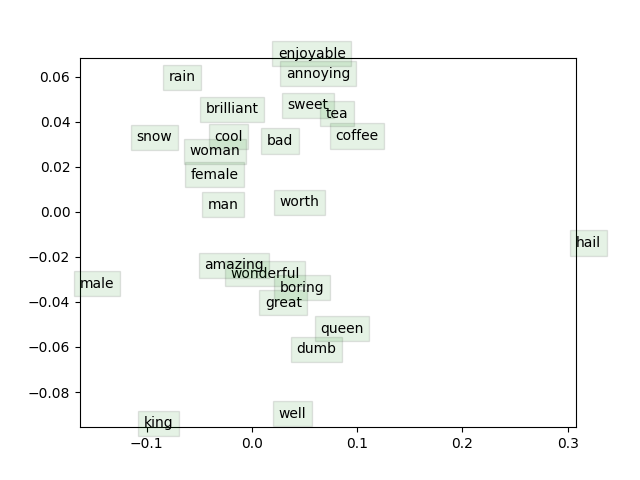
\includegraphics[scale=0.5]{images/word_vectors.png}
	\caption{A plot of the resulting word vectors}
\end{figure}
\begin{figure}[h]
	\centering
	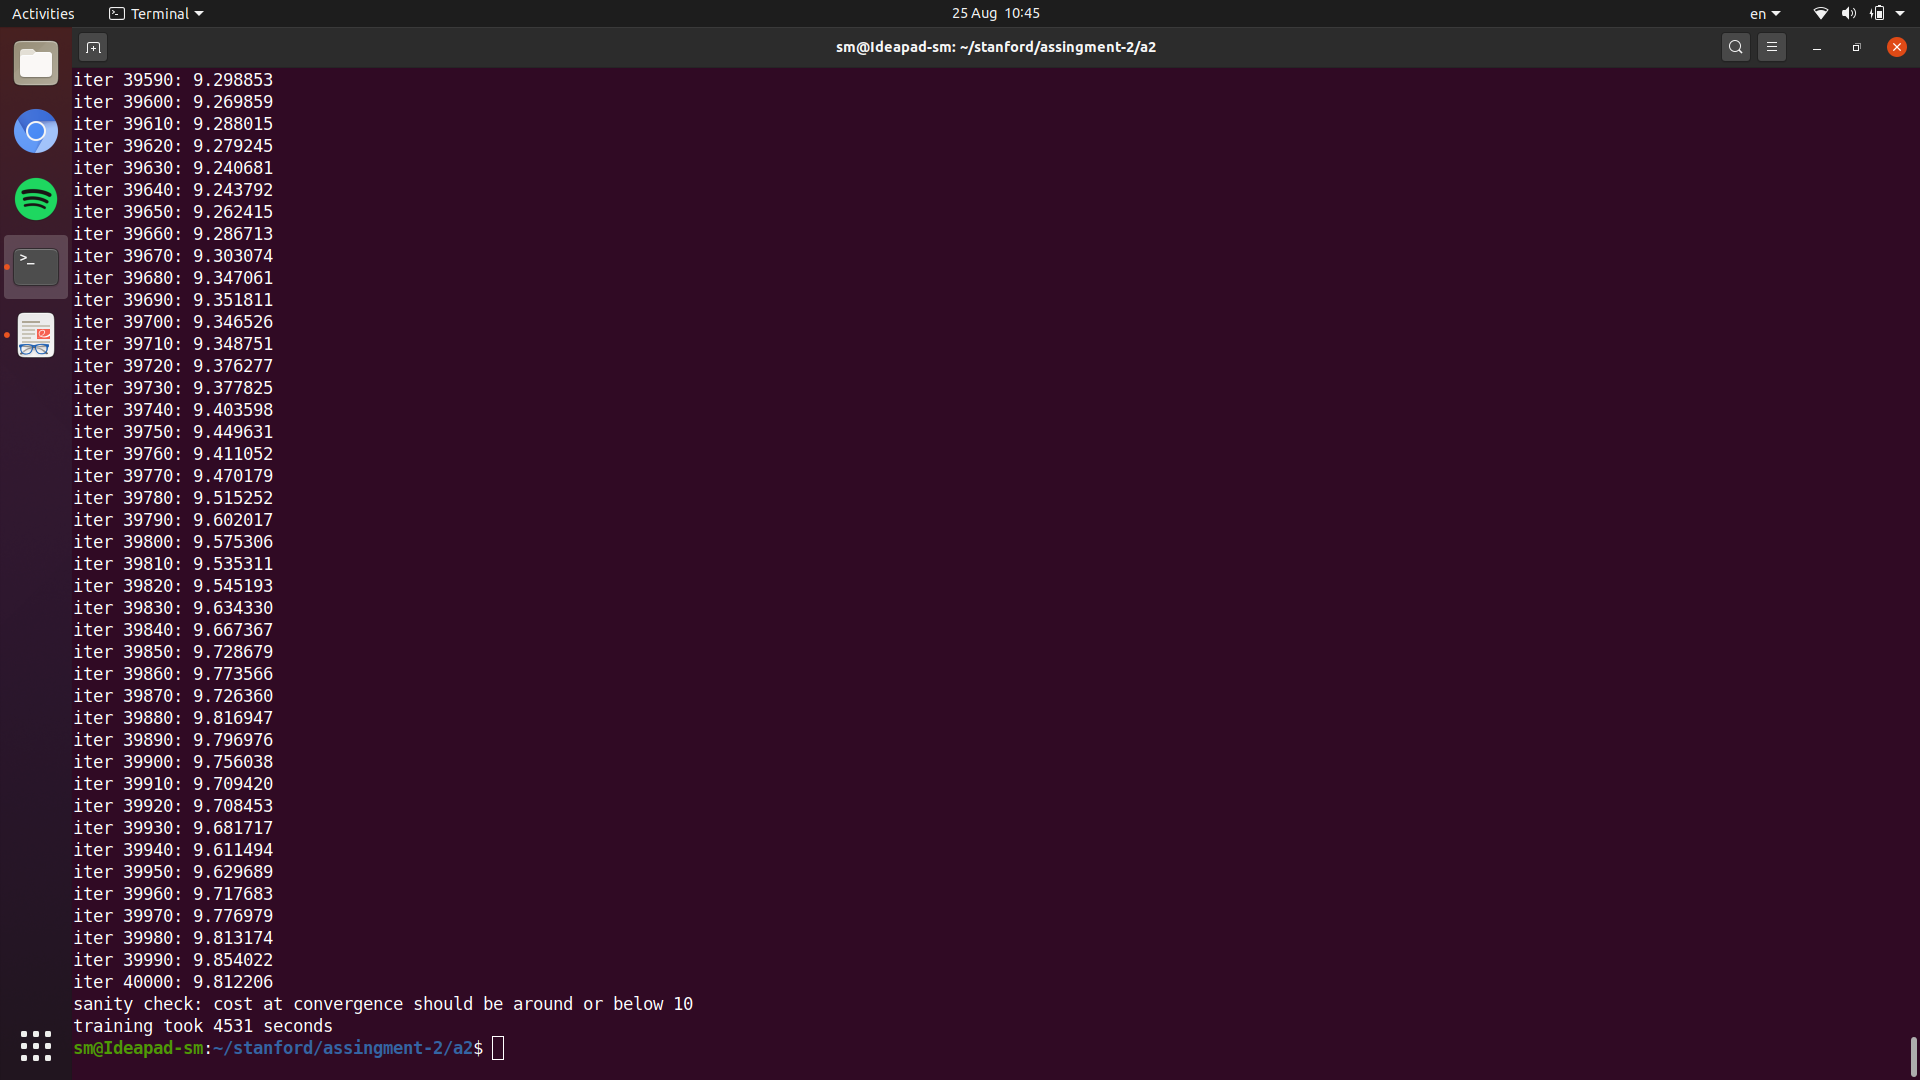
\includegraphics[scale=0.2]{images/time_and_loss.png}
	\caption{The time needed to train and output loss}
\end{figure}

\end{document}
